\section{Shortest Paths}\label{sec:1}

\subsection{Preliminaries on Graphs}\label{subsec:1.1}
An {\bf (undirected) graph} $G$ is a pair $(V, E)$, where $E$ is a set of 
unordered pairs of elements in $V$. The elements of $V$ are called {\bf vertices}
or {\bf nodes}; the elements of $E$ are called {\bf edges}. 

Let $u, v \in V$ and let $e = uv \in E$ be an edge. 
\begin{itemize}
    \item We say that $e$ is {\bf incident} to $u$ and $v$. 
    \item The vertices $u$ and $v$ are said to be {\bf adjacent}.
    \item We call $u$ and $v$ the {\bf endpoints} of $e$. 
\end{itemize}
By default, we assume that there are no parallel edges (i.e. two
edges $e = uv$ and $e' = u'v'$ in $E$ with $\{u, v\} = \{u', v'\}$) 
and no loops (i.e. an edge $e = uv \in E$ with $u = v$).

For distinct $u, v \in V$, a {\bf $u, v$-path} is a sequence of vertices 
$w_1, \dots, w_k$ such that $w_1 = u$, $w_k = v$, and $w_i w_{i+1} \in E$ 
for all $i = 1, \dots, k-1$.  

For example, consider the following graph $G = (V, E)$ with 
vertices $V = \{v_1, v_2, v_3, v_4\}$ and edges $E = \{v_1v_2, v_1v_4, v_2v_3, 
v_2v_4, v_3v_4\}$. 

\begin{center}
    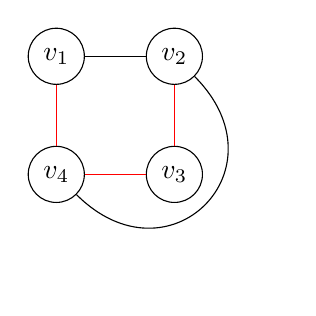
\begin{tikzpicture}[node distance={15mm}, main/.style = {draw, circle}] 
        \node[main] (1) {$v_1$}; 
        \node[main] (2) [right of=1] {$v_2$};
        \node[main] (3) [below of=2] {$v_3$}; 
        \node[main] (4) [left of=3] {$v_4$};

        \draw (1) -- (2);
        \draw [draw=red] (1) -- (4);
        \draw [draw=red] (2) -- (3);
        \draw (2) to [out=315, in=315, looseness=2] (4);
        \draw [draw=red] (3) -- (4);
    \end{tikzpicture} 
\end{center}
\vspace{-0.5cm}

The lines in red form a $v_1, v_2$-path, namely $v_1, v_4, v_3, v_2$. 
Another $v_1, v_2$-path can be obtained by simply traversing the edge $v_1v_2$. 

A {\bf cycle} in $G$ is a sequence of vertices $w_1, \dots, w_{k+1}$ 
such that $w_i w_{i+1} \in E$ for all $i = 1, \dots, k$, the vertices 
$w_1, \dots, w_k$ are all distinct, and $w_1 = w_{k+1}$.

Finally, a graph $G$ is {\bf connected} if for any pair of distinct vertices 
$u, v \in V$, there exists a $u, v$-path in $G$. 

\subsection{Shortest Paths Problem}\label{subsec:1.2}
Given a \emph{directed} graph $G = (V, E)$ with edge lengths $\ell_e \geq 0$
for each $e \in E$ and a distinguished start vertex $s \in V$, we wish 
to find shortest paths from $s$ to every other vertex in $V$. Note that 
when we work with directed graphs, we will denote the directed edges 
with $(v_1, v_2)$ as opposed to $v_1 v_2$ in the case of undirected graphs, where 
the order of the vertices did not matter. 

The {\bf length} of a path $P$ given by the sequence $w_1, \dots, w_k$ 
is given by 
\[ \ell(P) := \sum_{i=1}^{k-1} \ell_{(w_i, w_{i+1})} = \sum_{e\in P} \ell_e, \] 
where the second sum makes sense because there are no parallel edges. 
Then the {\bf shortest-path distance} from $s$ to a vertex $u \in V$ is 
defined to be
\[ d(u) := \min_{\text{$s,u$-paths $P$}} \ell(P). \] 
For example, we can consider the following instance of an undirected graph 
with given edge lengths and starting vertex $s = v_1$. 

\begin{center}
    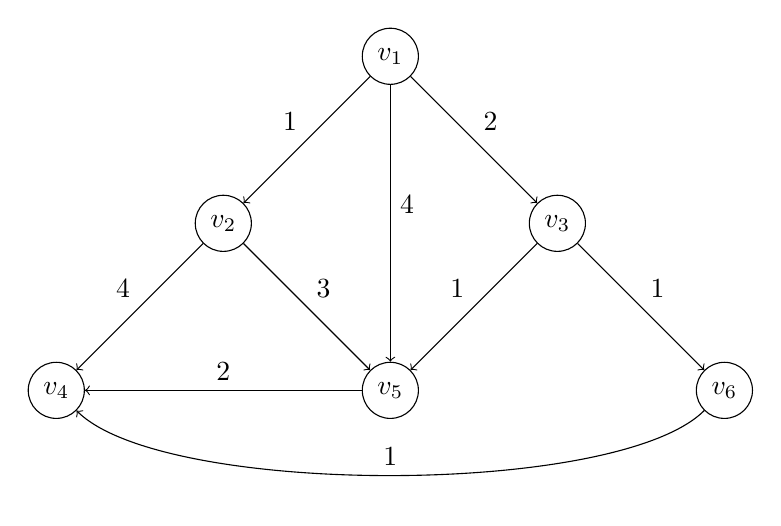
\begin{tikzpicture}[node distance={30mm}, main/.style = {draw, circle}] 
        \node[main] (1) {$v_1$}; 
        \node[main] (2) [below left of=1] {$v_2$};
        \node[main] (3) [below right of=1] {$v_3$}; 
        \node[main] (4) [below left of=2] {$v_4$};
        \node[main] (5) [below left of=3] {$v_5$};
        \node[main] (6) [below right of=3] {$v_6$};

        \draw[->] (1) -- node[midway, above left] {1} (2);
        \draw[->] (1) -- node[midway, above right] {2} (3);
        \draw[->] (1) -- node[midway, above right] {4} (5);
        \draw[->] (2) -- node[midway, above left] {4} (4);
        \draw[->] (2) -- node[midway, above right] {3} (5);
        \draw[->] (3) -- node[midway, above left] {1} (5);
        \draw[->] (3) -- node[midway, above right] {1} (6);
        \draw[->] (5) -- node[midway, above] {2} (4);
        \draw[->] (6) to [out=225, in=315, looseness=0.5] node[midway, above] {1} (4);
    \end{tikzpicture} 
\end{center}
\vspace{-0.5cm}
In this case, we have $d(v_2) = 1$, since the only possible path from 
$v_1$ to $v_2$ is by taking the edge $(v_1, v_2)$. There are multiple
paths from $v_1$ to $v_5$; the shortest one is $v_1, v_3, v_5$ giving 
$d(v_5) = 3$. 

Note that we always set $d(s) = 0$. We now make some observations: 
\begin{enumerate}[(i)]
    \item If $(u, v) \in E$, then $d(v) \leq d(u) + \ell_{(u,v)}$, since 
    such an $s, v$-path is always an option.
    \item For every $v \in V$ distinct from $s$, there exists $w \in V$ 
    such that $d(v) = d(w) + \ell_{(w, v)}$ and $(w, v) \in E$. This can 
    be seen by chopping off the last edge from a shortest path from $s$ to $v$.
\end{enumerate}
